\documentclass{article}

% if you need to pass options to natbib, use, e.g.:
%     \PassOptionsToPackage{numbers, compress}{natbib}
% before loading neurips_2019

% ready for submission
% \usepackage{neurips_2019}

% to compile a preprint version, e.g., for submission to arXiv, add add the
% [preprint] option:
%     \usepackage[preprint]{neurips_2019}

% to compile a camera-ready version, add the [final] option, e.g.:
     \usepackage[final]{project-report}

% to avoid loading the natbib package, add option nonatbib:
%     \usepackage[nonatbib]{neurips_2019}

\usepackage[utf8]{inputenc} % allow utf-8 input
\usepackage[T1]{fontenc}    % use 8-bit T1 fonts
\usepackage{hyperref}       % hyperlinks
\usepackage{url}            % simple URL typesetting
\usepackage{booktabs}       % professional-quality tables
\usepackage{amsfonts}       % blackboard math symbols
\usepackage{nicefrac}       % compact symbols for 1/2, etc.
\usepackage{microtype}      % microtypography
% \usepackage[round]{natbib}
\usepackage{graphicx}
\usepackage{array}

\bibliographystyle{unsrtnat}

\title{Detecting Signs of Depression in Social Media Texts}

% The \author macro works with any number of authors. There are two commands
% used to separate the names and addresses of multiple authors: \And and \AND.
%
% Using \And between authors leaves it to LaTeX to determine where to break the
% lines. Using \AND forces a line break at that point. So, if LaTeX puts 3 of 4
% authors names on the first line, and the last on the second line, try using
% \AND instead of \And before the third author name.

\author{%
  Kaishuo Wang\\
  School of Electrical Engineering and Computer Science (EECS)\\
  University of Ottawa\\
  Ottawa, ON, Canada \\
  \texttt{kwang126@uottawa.ca} \\
  % examples of more authors
  % \And
  % Coauthor \\
  % Affiliation \\
  % Address \\
  % \texttt{email} \\
  % \AND
  % Coauthor \\
  % Affiliation \\
  % Address \\
  % \texttt{email} \\
  % \And
  % Coauthor \\
  % Affiliation \\
  % Address \\
  % \texttt{email} \\
  % \And
  % Coauthor \\
  % Affiliation \\
  % Address \\
  % \texttt{email} \\
}

\begin{document}

\maketitle

\begin{abstract}
  This report outlines an improved approach to detect signs of depression in social media posts, as part of the LT-EDI-ACL-2022 shared task. The project contains four key systems: firstly, a fine-tuned BERT model for generating sentiment features, secondly, a classification system concatenating BERT sentence embeddings and additional emotion features, thirdly, a prompt-based classification system, and finally, an ensemble system combining predictions with weighted scores. Leveraging the publicly available LT-EDI-ACL-2022 shared task dataset, the training and evaluation involve 8891 sentences, facilitating nuanced classification into \emph{not depression}, \emph{moderate}, and \emph{severe}. Results indicate the effectiveness of this improved strategy, with the ensemble system demonstrating notable improvements. These findings suggest practical applications in screening and identifying depression from vast social media data, contributing to the advancement of natural language processing in mental health contexts. The code for this project can be found at: \emph{\url{https://github.com/KaishuoWang/Depression-Detection/tree/main}}.
\end{abstract}

\section{Introduction}

Depression, a pervasive mental health concern, poses significant challenges to individuals and society at large. Left untreated, it can lead to severe consequences, holding off early detection and intervention which are crucial for mitigating its impact. Leveraging the vast landscape of social media data to identify signs of depression represents a novel and promising avenue for reaching at-risk individuals. This notion forms the foundation of the LT-EDI-ACL-2022 shared task 4\footnote{\url{https://sites.google.com/view/lt-edi-2022/tasks?authuser=0}} — an initiative aimed at detecting indicators of depression from social media posts. This report delves into the methodologies employed to address this task, where the classification of the textual content contains three distinct categories — \emph{not depression}, \emph{moderate}, and \emph{severe}. The overarching goal is to facilitate the identification of signs of depression from social media texts through automated methods.

The present project expands upon the framework proposed by \citep{wang2022nycu_twd}, introducing significant modifications and enhancements across three crucial dimensions. The initial modification involves the adoption of a fine-tuned BERT model, departing from the conventional VADER approach, to extract richer sentiment features. The fine-tuning process, conducted on sentiment analysis datasets, enhances the model's adaptability to the unique intricacies of the task. Leveraging contextual embeddings from BERT, known for their ability to capture nuanced emotions, proves instrumental in surpassing the performance of the traditional lexicon-based VADER method \citep{saha2022vader}. Following this, a classification system is constructed utilizing another BERT model. During the classification process, sentence embeddings are combined with additional features derived from the preceding sentiment analysis step. This collaborative approach aims to yield a more precise prediction by capitalizing on both the power of contextual embeddings and the nuanced sentiment features extracted from the text.

The second modification introduces the exploration of prompt-based classification, inspired by \citep{deng2022beike}. A carefully crafted prompt, \emph{"The level of depression in the following tweet is {MASK}"}, tasks the model with accurately filling the \emph{MASK} using one of the predefined depression levels. This strategic use of prompts, coupled with BERT fine-tuning, minimizes the need for extensive task-specific architecture modifications, potentially leading to more efficient and accurate classification.

The third modification involves the incorporation of zero-shot classification, bringing several advantages to the project. Zero-shot classification allows the model to generalize and classify instances that were not seen during training, making it particularly useful in scenarios where novel or unexpected expressions of depression may emerge. Despite exploring various publicly available zero-shot classification models, none demonstrated satisfactory results, prompting the decision to fine-tune a dedicated model using the project's data to ensure optimal performance.

Finally, an ensemble system is introduced to amalgamate predictions from the aforementioned systems. This ensemble system utilizes the normalized F1 score of each model on the testing set as a weight, contributing to the derivation of the ultimate prediction.

In summary, this report presents a comprehensive framework for identifying signs of depression in social media texts. During the evaluation phase, this approach showcases a notable performance leap forward from the original work (obtained 0.8044 in macro F1-score).

\section{Related Work}

\citep{wang2022nycu_twd} introduced a comprehensive framework that harnesses sentiment analysis and sentence embeddings to capture both emotional and semantic dimensions of textual content. The system begins by processing input text, generating sentiment features through the VADER tool and creating sentence embeddings using a pre-trained model. The subsequent stages involve employing three distinct methods to model various aspects of the text, with Ensemble techniques introduced to seamlessly integrate the resulting predictions.

In the first method, concatenated sentence embeddings and sentiment feature embeddings serve as input, and to address imbalanced data, SMOTE and CondensedNearestNeighbour techniques are applied. The classification stage leverages LightGBM and XGBoost. In contrast, the second method exclusively utilizes sentence embeddings as input, employing a multilayer perceptron model as a classifier. The third system follows a similar approach to the first, utilizing concatenated sentence embeddings and sentiment feature embeddings as input, and employing a multilayer perceptron model for classification.

Once predictions are harvested from each method, the ensemble system steps up, orchestrating a seamless fusion of these diverse predictions with manually assigned weights.

\section{Dataset}

To rigorously evaluate these modifications, the project utilizes the publicly available LT-EDI-ACL-2022 dataset provided by \citep{kayalvizhi2022findings}. The dataset comprises 8891 sentences for training, 4496 for validation, and 3245 for testing. Each sample has a PID, a text and a label indicating the depression level. Table ~\ref{table1} shows some examples from this dataset.

\begin{table}[h]
  \caption{Samples from the depression dataset}
  \label{table1}
  \centering
  \renewcommand{\arraystretch}{1.5} % Default value: 1
  \begin{tabular}{lp{8cm}p{3cm}p{3cm}}
    \toprule
    \textbf{PID} & \textbf{Text} & \textbf{Label} \\
    \midrule
    train-pid-1 & Waiting for my mind to have a breakdown once the “New Year” feeling isn’t there anymore : I don’t know about anyone else, but I’m a little bit worried that I’ll go back to being depressed in a few days time or something. Last year, I tried not to have any breakdowns for the start of 2019. A mere 10 days later, I broke down crying. I wasn’t the same for that entire year. Up until December, where I was ok that month. Now I just wait... it’s a weird way to act and feel, but it feels a bit normal.  & moderate     \\ \hline

    train-pid-2 & Words can't describe how bad I feel right now: I just want fall asleep forever. & severe \\ \hline

    train-pid-3 & Is anybody else hoping the Coronavirus shuts everybody down? & not depression  \\
    \bottomrule
  \end{tabular}
\end{table}

The dataset \citep{Berenstein} employed for fine-tuning the BERT model to generate emotion scores, comprises 22,027 samples in the training set, 13,487 samples in the testing set, and 9,441 samples in the validation set. The dataset encompasses five distinct labels, namely \emph{extremely negative}, \emph{negative}, \emph{neutral}, \emph{positive}, and \emph{extremely positive}, offering a comprehensive spectrum of emotional states. This dataset aligns with the nature of social media content prevalent in the depression detection dataset which helps to enhance the model's adaptability to the nuances of social media language. Table ~\ref{table2} shows some examples from this dataset.

\begin{table}
  \caption{Samples from the sentiment analysis dataset}
  \label{table2}
  \centering
  \renewcommand{\arraystretch}{1.5} % Default value: 1
  \begin{tabular}{p{10cm}p{3cm}}
    \toprule
    \textbf{Text} & \textbf{Label} \\
    \midrule
    Thank you to all supermarket workers Please stay safe  & Extremely Positive \\ \hline
    
    Covid 19 M sia supermarket provides picture guides to help confused husbands buy groceries during lockdown & Positive \\ \hline
    
    It was a toilet paper pandemic more than a Coronavirus pandemic in my opinion & Neutral \\ \hline

    You never know this COVID-19 thing is serious until you queue outside supermarket..In Naivas and guys getting in lots of 10 only... & Negative \\ \hline

    A worker from the supermarket down the street has died from COVID 19 He had recently visited family in the UK Very sad & Extremely Negative \\
    \bottomrule
  \end{tabular}
\end{table}

\section{Methodology}

The proposed approach consists of three methods and an ensembling system. Figure 1 illustrates the pipeline of this approach.

\begin{figure}[t]
    \centering
    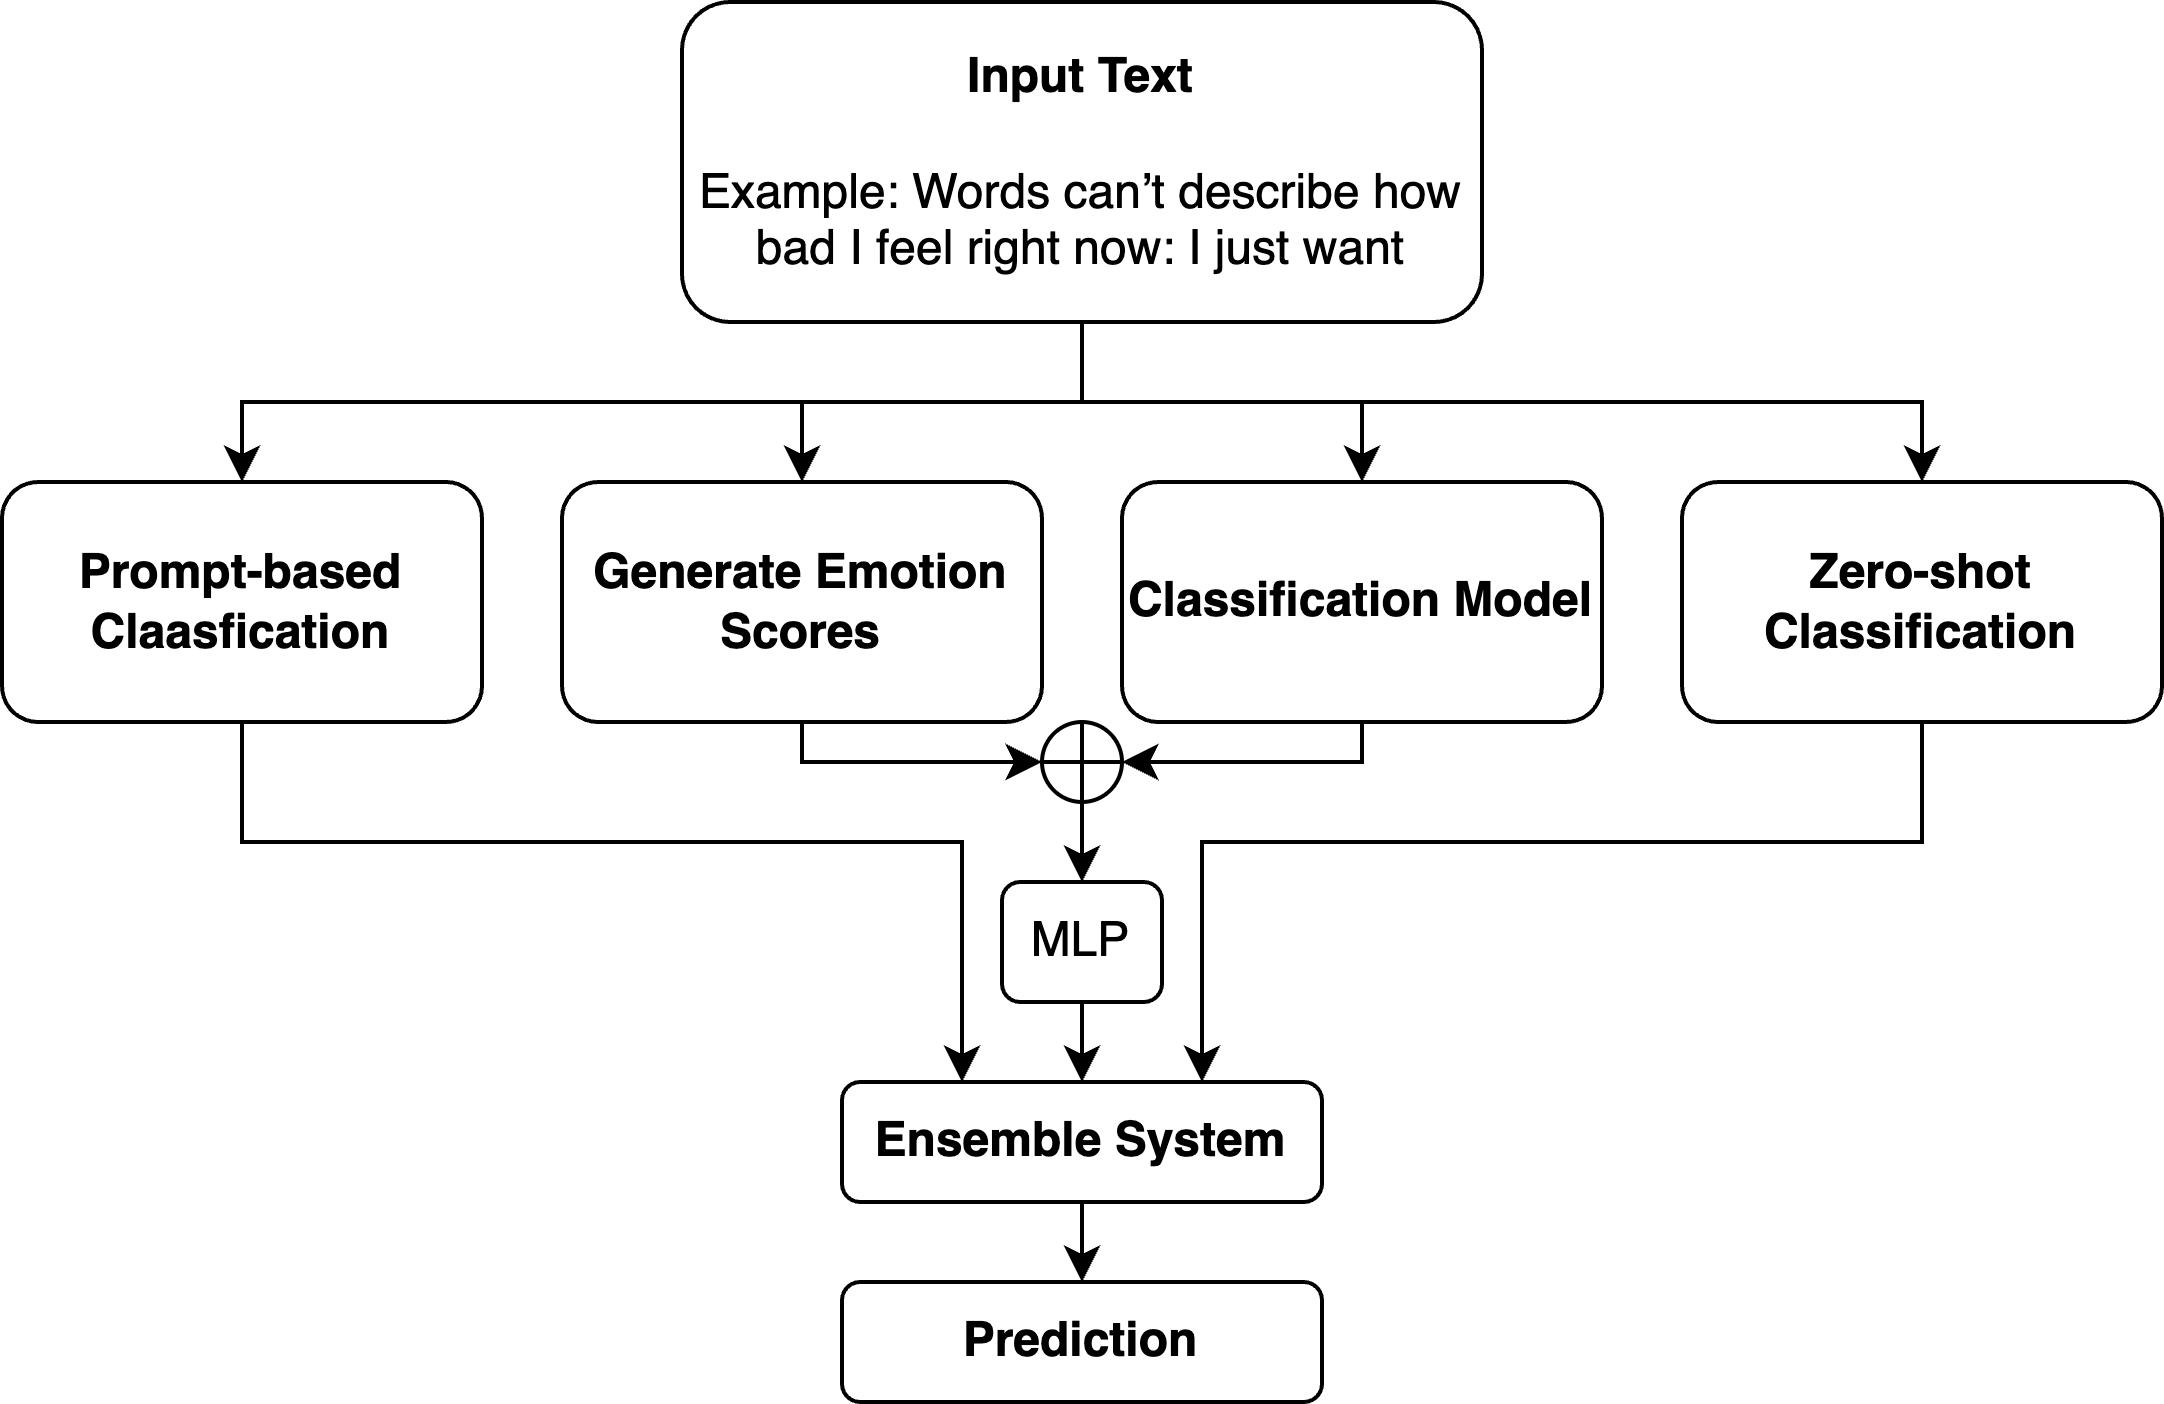
\includegraphics[width=10cm]{system-structure.png} % modified by Karol Kozioł
    \caption{Structure of the proposed framework}
\end{figure}

\subsection{Traditional Classification}

The methodology for fine-tuning BERT for depression detection using a traditional classification approach involves a multi-step process. Firstly, the fine-tuning process for the sentiment analysis component involved the utilization of the \emph{bert-base-uncased} model. The selection of this model was driven by a careful consideration of optimizing inference time, a crucial factor in the efficiency of the subsequent classification tasks. In a departure from conventional preprocessing practices, no alterations were made to the training data. This decision was made intentionally to preserve the raw and unfiltered nature of social media language, recognizing its inherently nuanced and informal structure. The sentiment analysis dataset chosen for fine-tuning classifying text into five distinct categories, ranging from \emph{extremely negative} to \emph{extremely positive}. This detailed classification schema was instrumental in enabling the model to capture a broad spectrum of sentiments present in social media content. The inclusion of categories beyond the typical positive-neutral-negative triad provided a more granular understanding of the emotional nuances embedded in the text.

After that, the input texts are fed into the pre-trained BERT model to extract contextual embeddings, capturing the nuanced semantics of the text. Subsequently, the emotion scores derived from the sentiment analysis are concatenated with the BERT sentence embeddings. The combined feature set, comprising both contextual embeddings and emotion scores, is then passed through a Multilayer Perceptron (MLP) model for the classification task. During the training phase, the model learns to associate the concatenated features with the corresponding depression severity labels, adapting its weights and biases to effectively capture the complex relationships within the data. This methodology aims to leverage the strengths of BERT's contextual embeddings and sentiment analysis for robust depression detection through a traditional classification framework.

\subsection{Prompt-based Classification}

In the prompt-based classification, a meticulously crafted prompt served as the linchpin: "The level of depression in the following tweet is {}." This prompt assumed a critical role as a structured template, guiding the model to complete the sentence with one of the predetermined categories – "not depressed," "moderately depressed," or "severely depressed." The core principle underlying this approach lies in tapping into the contextual understanding embedded within the pre-trained BERT model. Through the iterative fine-tuning process on the training dataset, the model cultivated a nuanced understanding of linguistic patterns indicative of varying degrees of depression in social media posts.

This prompt-based strategy was formulated to leverage the innate capabilities of BERT, exploiting its contextual awareness to discern subtle linguistic cues associated with distinct levels of depression. In the context of this project, the model of choice was \emph{roberta-large}, an evolution of the traditional BERT model. \emph{roberta-large} implemented modifications in the training process, including the utilization of larger mini-batches and the removal of the next sentence prediction objective. These adjustments have been empirically proven to enhance model generalization and training efficiency\citep{liu2019roberta}.

Beyond these modifications, the \emph{roberta-large} model's augmented capacity, attributed to its larger architecture, positions it favourably to capture more intricate linguistic nuances. The decision to incorporate \emph{roberta-large} into the methodology aligns with the project's objective of achieving a nuanced and contextually aware classification of depression levels in social media posts, leveraging the state-of-the-art capabilities embedded within this advanced transformer-based model.

\subsection{Zero-shot Classification}

The incorporation of the zero-shot classification approach involved fine-tuning a natural language inference (NLI) model, adding a layer of complexity and adaptability to the depression detection project. 

Initially, the dataset was prepared for NLI by executing a transformation process. This process involved converting the original dataset into the NLI format, which incorporated two labels: “entailment” and “contradiction.” The prompt from the prompt-based classification approach was repurposed in this transformation step. The original data was augmented with the NLI format by combining the text with the prompt. To create diverse instances, the mask in the prompt was filled with both the true label and a randomly selected incorrect label. This augmentation process introduced a nuanced perspective to the NLI model, allowing it to learn from instances where the depression level was correctly or incorrectly associated with the given text.

Following the dataset transformation, the NLI model was fine-tuned to adapt it specifically to the requirements of the depression detection task. This fine-tuning process was crucial in enabling the model to recognize and understand the intricate relationships between the textual content and the corresponding depression labels. Zero-shot classification empowers the model to make predictions on instances that were not encountered during the training phase, a capability particularly beneficial in scenarios where novel expressions of depression emerge in social media texts.

\subsection{Ensemble System}

The ensemble system, a pivotal component of this framework, is meticulously designed to synthesize predictions from multiple sub-systems. Specifically, the ensemble system leverages the normalized F1 score derived from each of the previously outlined approaches as a weight factor. These weights, reflective of the individual performance of each approach, are instrumental in assigning appropriate significance to the predictions generated by the respective systems. Upon obtaining the normalized F1 scores, they multiplied with the predicted probabilities from each system. The weighted probabilities are then aggregated, producing a composite set of probabilities that encapsulates the collective predictive power of the individual systems. The final step involves applying the \emph{argmax} function to the aggregated probabilities, facilitating the selection of the most probable label.
\begin{equation}
    \centering
    \label{formula1}
    P = argmax(P_1 \times w_1 + P_2 \times w_2 + P_3 \times w_3)
\end{equation}
where $P_1$, $P_2$, and $P_3$ are the probabilities calculated by each system, and $w_1$, $w_2$, and $w_3$ are the weight of each system.

This judicious integration of normalized F1 scores as weights ensures that the ensemble system not only considers the predictive capabilities of each approach but also factors in their relative strengths, allowing the ensemble model to adjust the impact of each prediction on the overall outcome. Thereby enhancing the robustness and reliability of the ultimate depression level classification for social media posts.

\section{Results}

The performance of each method is shown in Table ~\ref{table3}. \footnote{The result of NUCY\_TWD can be found at \url{https://github.com/wywyWang/Depression-Detection-LT-EDI-ACL-2022}}

\begin{table}[]
    \caption{Experiment Results}
    \label{table3}
    \centering
    \renewcommand{\arraystretch}{1.5} % Default value: 1
    \begin{tabular}{l|c|c|c}
        \toprule
        \textbf{Method} & \textbf{Accuracy} & \textbf{Weighted F1} & \textbf{Macro F1} \\
        \midrule
        NYCU\_TWD & 0.6330 & 0.6419 & 0.5830 \\
        \midrule \midrule
        Classification (with emotion features) & 0.7679 & 0.7686 & 0.7278 \\ \hline
        Zero-shot Classification & 0.7411 & 0.7410 & 0.7410 \\ \hline
        Prompt-based Classification & 0.6743 & 0.6160 & 0.3786 \\ 
        \midrule \midrule
        Classification + Prompt-based Classification & \textbf{0.8453} & \textbf{0.8488} & \textbf{0.8044} \\ \hline
        Classification + Zero-shot Classification & 0.8351 & 0.8358 & 0.7909 \\ \hline
        \multicolumn{1}{m{7cm}|}{Classification + Prompt-based Classification + Zero-shot Classification} & 0.8351 & 0.8358 & 0.7909 \\
        \bottomrule
    \end{tabular}
\end{table}

\subsection{Traditional Classification}

The traditional classification approach, leveraging fine-tuned BERT for sentiment analysis, yielded a noteworthy macro F1 score of 0.7278. This marked improvement over the original paper's F1 score of 0.5830 showcases the effectiveness of transitioning from lexicon-based sentiment analysis to contextual embeddings. The BERT model's ability to capture nuanced emotions in social media texts played a crucial role in achieving higher accuracy.

\subsection{Zero-shot Classification}

The zero-shot classification approach stands out with an impressive achievement, securing the highest macro F1 score of 0.7410 among all single methods. This outcome serves as compelling evidence for the effectiveness of the method employed. The substantial success in attaining such a high F1 score underscores the robustness and potency of the zero-shot classification approach, positioning it as a noteworthy solution for the task at hand. These results strongly support the notion that this method holds promise as a reliable and effective choice in addressing the challenges associated with the classification task.

\subsection{Prompt-based Classification}

The prompt-based classification approach, employing fine-tuned BERT with a structured prompt, resulted in a macro F1 score of 0.3786. While this approach demonstrated slightly lower performance compared to the traditional classification, it offered a valuable alternative, eliminating the need for extensive task-specific architecture modifications.

\subsection{Ensemble system}

The amalgamation of predictions from both traditional and prompt-based classification approaches resulted in the ensemble system emerging as the most successful, achieving a macro F1 score of 0.8044. The superior performance of the ensemble can be attributed to the complementary strengths of each individual system. The weighted combination of predictions, guided by normalized F1 scores on the testing set, underscores the effectiveness of integrating diverse strategies to create a more robust and accurate depression detection model.

However, it was observed that the integration of all three methods together yielded a slightly inferior result. This may be attributed to the correlation of errors, indicating that the zero-shot classification approach might be making similar mistakes as the traditional classification approach. When combined in an ensemble, these errors appear to reinforce each other, resulting in a less diverse and less robust ensemble. Consequently, the zero-shot classification approach will not be included in the final system.

\section{Conclusion}

In conclusion, this project aimed to enhance the detection of signs of depression in social media texts by leveraging advanced natural language processing techniques. The modifications made to the initial method proposed by \citep{wang2022nycu_twd} yielded promising results, demonstrating the effectiveness of our approach.

The experiments proved that the integration of a fine-tuned BERT model for sentiment analysis, as opposed to VADER, provided richer sentiment features, enhancing nuanced emotion capture. Additionally, we introduced prompt-based classification inspired by \citep{deng2022beike}, without the need for extensive task-specific architecture modifications.

Our ensemble system, combining traditional and prompt-based classifications, outperformed individual approaches with a macro F1 score of 0.8044. This approach demonstrated the complementary strengths of the two methods, with normalized F1 scores serving as adaptive weights. Moreover, comparing our framework's performance to the original paper's results, it is evident that our approach significantly outperformed their macro F1 score of 0.5830. This project contributes to advancing mental health detection through social media analysis, offering a robust and practical solution for early identification and intervention.

\clearpage

\section*{Disclosure}

This project is not part of other projects. I am trying to replicate and improve the work of \citep{wang2022nycu_twd}.

\bibliography{references}

\end{document}
